% Author: CSC Officers
\documentclass[11pt]{article}
\usepackage[margin=0.7in]{geometry}
\usepackage{listings}   %
\usepackage{needspace}  %
\usepackage{color}      %
\usepackage{ifthen}     % 
\usepackage{graphicx}   %
\usepackage{../includes/csc}        %
\usepackage{tikz}       %
\usetikzlibrary{shapes} %
\usepackage{tabularx}   % for helping matchtabular (matching questions)
\usepackage{textcomp}	% So our quotes in code don't look like shit
\usepackage{longtable}
\usepackage{multicol}
\usepackage[usenames,dvipsnames]{pstricks}
\usepackage{epsfig}
\setlength{\columnsep}{12em}

\lstset{ %
basicstyle=\footnotesize\ttfamily,       % the size of the fonts that are used for the code
numbers=left,                   % where to put the line-numbers
stepnumber=1,                   % the step between two line-numbers. If it's 1 each line will be numbered
numbersep=5pt,                  % how far the line-numbers are from the code
showspaces=false,               % show spaces adding particular underscores
showstringspaces=false,         % underline spaces within strings
tabsize=4,		                % sets default tabsize to 4 spaces
language=C,
upquote=true,
columns=fixed
}

\ifthenelse{\isundefined{\isAnswerKey}}
{
    \newenvironment{answer}{\large\lstset{basicstyle=\tiny\ttfamily}\color{white} \small{Answer:}}{}
}
{
    \newenvironment{answer}{\large\lstset{basicstyle=\large\ttfamily}\color{red} \small{Answer:}}{}
}

% ----- Start matchtabular definition -----
\newcounter{matchleft}
\newcounter{matchright}
\newenvironment{matchtabular}{%
  \setcounter{matchleft}{0}%
  \setcounter{matchright}{0}%
  \tabularx{\textwidth}{%
    >{\leavevmode\hbox to 1.5em{\stepcounter{matchleft}\arabic{matchleft}.}}X%
    >{\leavevmode\hbox to 1.5em{\stepcounter{matchright}\alph{matchright})}}X% 
    }%
}{\endtabularx}
% ----- End matchtabular definition -----

\title{CSCI-142 Exam 1 Review}
\author{Computer Science Community}
\date{\today}

\makeatletter
\let\thetitle\@title
\let\theauthor\@author
\let\thedate\@date
\makeatother

\begin{document}
\header

\begin{enumerate}

\section*{History and Evolution of Programming Languages}

	\item Explain the relationship between machine language, assembly language, and high level languages.\\
\begin{answer}
\small{\textbf{Machine language} is a set of instructions that is executed directly as-is by the computer's CPU itself. This is considered the lowest level representation of a computer program, and, while it is possible to program directly in machine code, it is highly tedious and error prone, making higher level languages favorable. Writing machine code is typically only done when troubleshooting a system or when implementing extreme optimization.\\
\textbf{Assembly language} is also considered a low-level programming language, and, in particular, assembly usually has a near 1:1 relationship between the assembly code and the architechure's machine code instructions. Assembly languages are specific to a computer's architechture - for example, assembly code you write for your phone (almost certainly) wouldn't work on your laptop. An example of an assembly language is MIPS. Programming in assembly language (and lower) is commonplace in embedded systems work.
\\
Finally, \textbf{high level languages} are, in general, designed to be portable across many different architechtures. What separates the high level languages from their lower level counterparts is that, due to this fact, they require compiling, which translates your high-level code into a form which the machine can understand (which varies by architechture.) When people talk about programming languages, they are most often referencing one of the high level languages, unless otherwise specified. High level languages include C and C++, Python, and Java.}
\end{answer}


\section*{Differences in Language Paradigms}
	\item ahh

\section*{Programming In C}
	\item ahh

\section*{Modular Design and Development}
	\item ahh

\section*{Variables and Basic Data Types}

	\item List the 7 basic data types in C (not including the unsigned variants).

\begin{answer}
char, short, int, long, long long, float, double
\end{answer}

	\item There are at least two issues in the following code. What are they?

\begin{verbatim}
#include <stdio.h>

int main(void) {
    int numbers[] = { 3, 6, 4, 5, 14, 9 };
    int sum, i = 0;
    double average;
    for (; i < 6; ++i) {
        sum += numbers[i];
    }
    average = sum / 6;
    printf("%f", average);
    return 0;
}
\end{verbatim}

\begin{answer}
\begin{enumerate}
\item \texttt{sum} is not initialized to 0, so \texttt{sum} does not contain the actual sum of the numbers in the array.
\item Because \texttt{sum} and \texttt{6} are both of type \texttt{int}, integer division is performed, and \texttt{average} does not contain the expected average, but the floor of the average. Change that line of code to one of the following:
\begin{verbatim}
average = sum / 6.0;
\end{verbatim}
\begin{verbatim}
average = (double)sum / 6;
\end{verbatim}
\begin{verbatim}
average = sum / (double)6.0;
\end{verbatim}
\end{enumerate}
\end{answer}


	\item Examine the following program:

\begin{verbatim}
#include <stdio.h>

int main(int argc, char* argv[]) {
    int number = atoi(argv[1]);      // atoi parses int from str
    int found;
    do {
        int i;
        found = 1;
        --number;
        for (i = 2; i < number; ++i) {
            if (!(number % i)) {
                found = 0;
                break;
            }
        }
    } while (!found);
    printf("%d", number);
    return 0;
}
\end{verbatim}

\begin{enumerate}

\item What does this program do? What is the output of \texttt{./a.out 10}? Step through the program execution if it helps.

\begin{answer}
This program finds the largest prime number less than the first command line argument. \texttt{./a.out 10} sets \texttt{number} to 10. The first iteration of the do-while loop decrements \texttt{number} to 9, then the for loop tests all integers between 2 and 8 inclusive for one that divides into 9 evenly. It finds that \texttt{9 \% 3} equals 0, so \texttt{!(9 \% 3)} equals 1. Since 1 is not equal to 0, it enters the if statement and breaks out of the for loop. It continues the do-while loop, decrements \texttt{number} to 8, and finds 2 divides into 8 evenly. \texttt{number} is then decremented to 7, and all integers from 2 to 6 inclusive are tested to check if they divide into 7 evenly. None of them do (because 7 is prime), so the if statement isn't executed. \texttt{found} is now 1 at this point, making \texttt{!found} equal 0, which stops the loop, and 7 is then printed.
\end{answer}



\item Why can we write \texttt{if (!(number \% i))} instead of \texttt{if (number \% i == 0)}? (These statements are equivalent.)

\begin{answer}
If statements in C check whether their condition is not equal to 0, rather than if they are equal to a dedicated "true" value. If \texttt{number \% i} is 0 (that is, \texttt{number} is a multiple of \texttt{i}), then \texttt{!(number \% i)} will equal 1, which is not equal to 0, so the if condition will be satisfied. Comparison operators all produce 0 or 1, so here, \texttt{number \% i == 0} would evaluate to \texttt{0 == 0}, which evaluates to 1.
\end{answer}


\newpage
\item Rewrite the code using while loops in place of the do-while loop and the for loop.

\begin{answer}
\begin{verbatim}
#include <stdio.h>

int main(int argc, char* argv[]) {
    int number = atoi(argv[1]);      // atoi parses int from str
    int found = 0;
    while (!found) {
        int i; 
        found = 1;
        --number;
        i = 1; // Start one below the desired initial value, as i will be immediately incremented.
        while (i < number) {
            ++i;
            if (!(number % i)) {
                found = 0;
                break;
            }
        }
    }
    printf("%d", number);
    return 0;
}
\end{verbatim}

Note that we place the increment statement at the top of the loop body because if the loop body contained a \texttt{continue} statement, the increment statement will always be executed, unlike if the increment statement were placed at the bottom. Because this code does not include a \texttt{continue} statement, initializing \texttt{i} to 2 and placing the increment statement at the bottom of the loop body will also produce the correct behavior.
\end{answer}

\end{enumerate}



\section*{Control Structures}
	\item ahh

\section*{Operators}
	\item ahh

\section*{Arrays}

	\item ahh

\section*{I/O}

	\item ahh

\section*{C Pre-processor}

	\item What is the value of \texttt{i}?
\begin{verbatim}
#define THING1 40
#define THING2 32

#if THING1 < THING2
#define THING3 5
#elif THING2 < THING1
#define THING3 6
#else
#define THING3 7
#endif

int i = THING3;
\end{verbatim}
\begin{answer}
6
\end{answer}


\section*{Memory and Program Layout}

	\item \textbf{Memory and Program Layout}

Label the sections of the program in memory

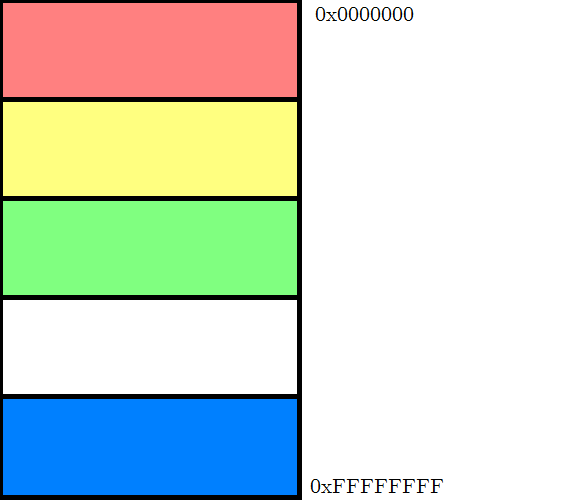
\includegraphics[width=50mm]{questions/programstructure.png}

\begin{answer}
red: text

yellow: data

green: heap

blue: stack
\end{answer}

\section*{Functions}

	\item ahh

\section*{Structs}

	\item ahh

\section*{Strings}

	\item ahh


\section*{Program Maintenance}

	\item ahh

\section*{C Pointers}

	\item ahh

\section*{Dynamic Storage}

	\item ahh


\end{enumerate}
\end{document}

Topics for this exam:
	- History and Evolution of Programming Languages
	- Differences in Language Paradigms
	- Programming Environments
	- Modular Design and Development
	- C: Variables, basic data types			DAKOTA/YAWAR
	- C: control structures, operators, arrays  YAWAR
	- C: basic I/O								YAWAR
	- C: basic CPP								DAKOTA
	- The OS: memory, program layout			DAKOTA
	- C: Functions, Structs, Strings			KATIE
	- Program Maintenance
	- C Pointers and Dynamic Storage			KATIE
